%This is the text for HNL searches

%Heavy Neutral Leptons (HNLs) are in general introduced to naturally explain neutrino masses and oscillations, giving masses to active neutrinos with Yukawa coupling, as for other leptons.  Since HNLs are gauge-singlet fermions they should have a Majorana mass term, which can (help to) explain: Smallness of neutrino masses, Baryon-antibaryon asymmetry in the Universe via Leptogenesis and Dark Matter (see section Sec.~\ref{}).

Heavy Neutral Leptons (HNLs) are the simplest extension envisaged to the SM:
%and in addition they can explain naturally the neutrino masses.
there are several specific models that predict the existence of HNLs, such as the $\nu$MSM~\cite{Asaka:2005pn}, Left-Right symmetric model~\cite{Pati:1974yy,Mohapatra:1974gc,Senjanovic:1975rk}, some SUSY scenarios~\cite{LopezFogliani:2005yw} and several others (see for instance ~\cite{Akhmedov:1998qx,Kersten:2007vk}). Particularly interesting are models predicting the existence of these particles below the electroweak breaking scale where they can be searched for experimentally. 
If the mass of HNLs is in the GeV region they can be produced in meson decays, such as $D_s^+\to \mu^+ N$. HNLs  decay by mixing with active neutrinos, %as shown for instance in Fig.~\ref{fig:Feynman}, 
where $U_{\ell}^2$ gives the mixing probability with an active neutrino of a specific flavour. Notice that the full process might violate Lepton Flavour and Lepton Number. 
%The impact of a possible discovery of HNLs in Particle Physics is therefore difficult to overestimate, since these particles might solve the main problems of the Standard Models and provide evidence for Lepton Number and Lepton Flavour Violation. 
HNLs have been searched for at colliders (see~\cite{Sirunyan:2018mtv,ATLAS:2012ak,Aaij:2014aba}). In addition, sensitivity studies have been performed for Future Circular Colliders~\cite{Blondel:2014bra,Drewes:2016jae,Antusch:2017pkq} (FCC). FCC has the possibility to set strong constraints on HNLs for masses above a few tens of GeV and below the $Z$ mass. In the region below 10 GeV the lifetime of HNLs becomes in general very long such that experiments with large fiducial volume, like those designed for searches for hidden sector particles, are optimal. 
Proposals for the LHC-based experiments FASER~\cite{Feng:2017uoz}, MATHUSLA~\cite{Curtin:2018mvb} and CODEX-b~\cite{Gligorov:2017nwh}, include sensitivity studies for HNLs. Their experimental signature  consists of isolated displaced vertexes. The critical parameters in these experiments are the size of their fiducial volume and the distance from the interaction point. These parameters have to be balanced with the level of background, and the possibility to measure momentum and identify the decay channels. While MATHUSLA has the best sensitivity among such experiments because of the large decay volume, it does not allow measuring decay channels, therefore HNL-signatures are indistinguishable from other hidden sector particles. On the other hand FASER, which allows measuring final states and masses, has a small fiducial volume and therefore a limited sensitivity. 

Proton Beam Dump experiments allow to achieve both things simultaneously, i.e.\ they have a relatively large acceptance while allow measuring mass and final states of the signal. 
The NA62 experiment at the SPS of CERN~\cite{Anelli:2005ju} is collecting data and its primary goal is to measure rare decays of $K$-mesons. 
In addition, NA62 plans to run in beam-dump mode (NA62$^{++}$), collecting roughly $10^{18}$ Protons On Target (POT) during Run3 (2021-2023). This would allow to set limits in a presently unconstrained region. 

SHiP~\cite{Anelli:2015pba} is a beam-dump experiment designed and optimized to search for Hidden Particles. It will take advantage of the high intensity proton beam of the Beam-Dump Facility~\cite{SHiP:2018yqc} (BDF) under study in the context of the Physics Beyond Collider study activity, that would allow starting data taking in Run 4 of the CERN accelerator schedule. SHiP will accumulate the full statistics of NA62$^{++}$ every few days, thanks to the larger acceptance and beam intensity ($2\times 10^{20}$ POT in 5 years). 
Figure XX in chapter YY shows the sensitivity as a function of the mass of HNLs and the mixing angle with active electron neutrinos ($U^2_{e}$), for various planned and proposed experiments.
%Figure~\ref{fig:sensitivity} shows the sensitivity as a function of the mass of HNLs and the mixing angle with active electron neutrinos ($U^2_{e}$) , for  various planned and proposed experiments~\cite{Beacham:2019nyx}. For LHC-based experiments the full exposure of the High-Luminosity phase is assumed.  
%Similar sensitivities are expected for the $U_{\mu}^2$, while the sensitivities for $U_{\tau}^2$ are in general roughly an order of magnitude worse below 10~GeV/$c^2$. 
%It should be emphasized that zero background is assumed for all experiments. This has been demonstrated for SHiP with full simulation studies,  while this assumption is still to be proven for MATHUSLA and CODEX-B. 
%Finally, in case of signal observation, the possibility to measure mass and decay channels at NA62$^{++}$ and SHiP would allow testing the compatibility between HNL parameters and neutrino oscillations and/or leptogenesis. In addition, the invariant mass would be a powerful tool, in case  more than one signal event is observed, to discard the possibility of underestimated background.
Note that also neutrino experiments thanks to the high proton intensity of the primary beam are competitive for searching HNLs in the near detectors, as demonstrated in \cite{Abe:2019kgx, Ballett:2019bgd, Arguelles:2019xgp}.

%\begin{figure}[htbp]
%    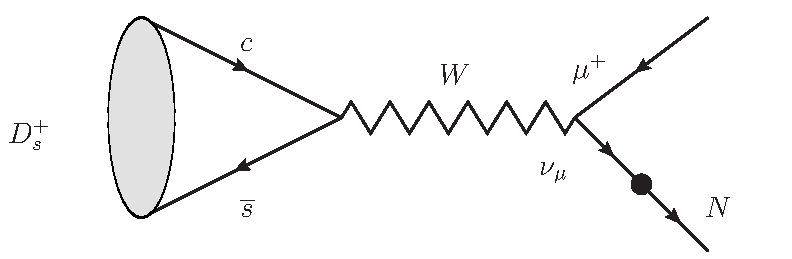
\includegraphics[scale=0.5]{\main/Neutrino/img/Ds2muN.pdf}
%    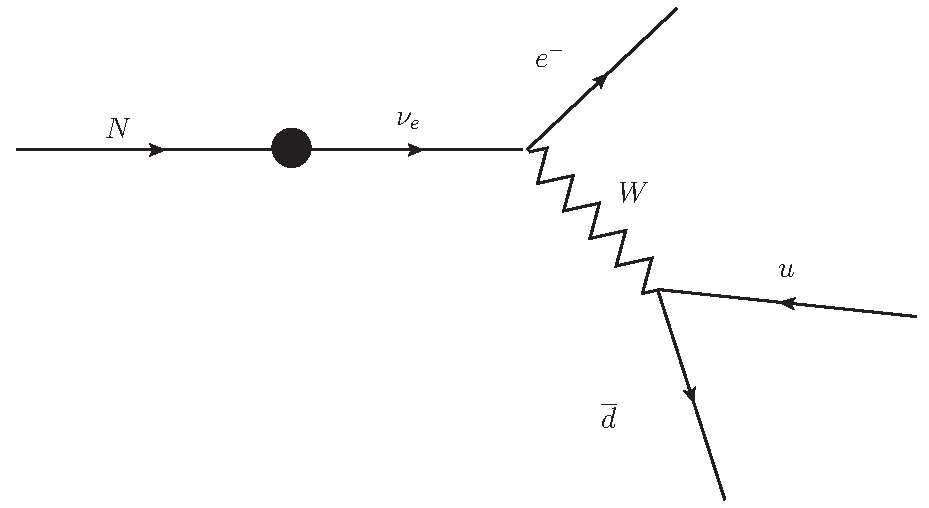
\includegraphics[scale=0.4]{\main/Neutrino/img/N2epi.pdf}
%    \caption{Example of Feynman diagrams for the production (left) and decay %(right) of HNLs.}\label{fig:Feynman}
%\end{figure}

%\begin{figure}[htbp]
%    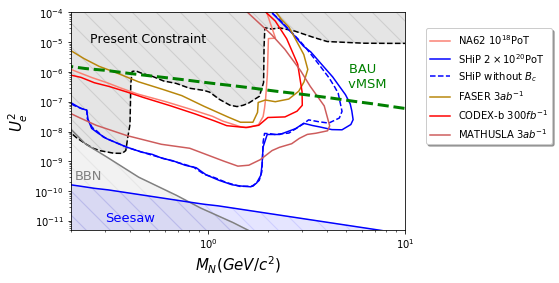
\includegraphics[scale=0.8]{\main/Neutrino/img/Sensitivity2.png}\\
%    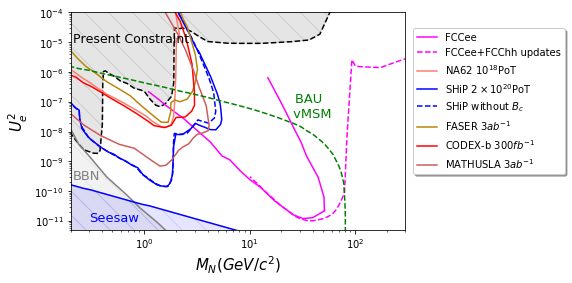
\includegraphics[scale=0.8]{\main/Neutrino/img/Sensitivity.png}
%    \caption{Sensitivity to HNLs as a function of mass and the mixing with active electron neutrinos ($U_e^2$), for different proposed experiments.}\label{fig:sensitivity}
%\end{figure}


